\section{Základní pojmy z teorie množin}
\label{sec:zakladni-pojmy-z-teorie-mnozin}

Teorie množin tvoří společně s logikou základ moderní matematiky. Jedno možné
přirovnání je, že množiny tvoří svět, který lze zkoumat pomocí logiky. Pojem
\uv{množina} (podobně jako i \uv{pravda} a \uv{lež} v logice) není možné v
teorii množin definovat, poněvadž je její základní stavební jednotkou. Stejně
jako všechny teorie současné matematiky je i teorie množin definována
\emph{axiomaticky}. Axiomy jsou logické výroky, které v dané teorii nelze
dokázat, a jsou a priori označeny za pravdivé. Jsou vlastně jakousi matematickou
verzí zázraku. Přestože znalost a porozumění axiomům teorie množin se považuje
za základ matematického vzdělání, jejich podoba je tomuto textu irelevantní a
zmiňovat je nebudeme. Snad kromě toho prvního, asi nejpřirozenějšího možného --
\uv{Existuje množina}.

Intuitivně asi každý matematik přemýšlí o množinách jako o souborech prvků,
které spolu nějakým způsobem souvisejí. Fakt, že prvek $x$ je součástí množiny
$A$, zapisujeme jako $x \in A$ a čteme \uv{$x$ náleží/je prvkem $A$} (symbol $
\in $ je pochroumané $e$ v angl. slově \textbf{e}lement). Když $B$ je množina,
jejíž každý prvek leží rovněž v $A$, pak píšeme $B \subseteq A$ a čteme tento
výrok jako \uv{$B$ je podmnožinou $A$} (případně \uv{$A$ je nadmnožinou $B$}).
Pomocí symbolu náležení ($ \in $) lze tento vztah též logicky vyjádřit jako
\[
 (B \subseteq A) \Leftrightarrow (x \in B \Rightarrow x \in A),
\]
tedy výrokem \uv{Když $x$ je prvkem $B$, pak $x$ je prvkem $A$.}

Naopak, fakt, že $y$ \emph{není} prvkem $A$, nezapisujeme krkolomně $\neg (y \in
A)$, nýbrž zkrátka $y \notin A$, a fakt, že $C$ \emph{není} podmnožinou $A$,
nepřekvapivě jako $C \nsubseteq A$. Potřebujeme-li zdůraznit, že $C$ je
podmnožinou $A$, ale není celou množinou $A$, píšeme $C \subsetneq A$.
\begin{warning}{}{mnozina-bez-poradi}
 Mnoho začínajících matematiků pěstuje slabě nepřesnou intuici o pojmu množiny.
 Totiž, množinu lze vnímat jako soubor prvků; není však radno chovat představu,
 že tyto prvky mají uvnitř množiny nějaké \uv{umístění} či \uv{pořadí} nebo
 \uv{četnost} či \uv{počet výskytů}. Že řada lidí z~počátku přisuzuje množinám a
 jejich prvkům tyto vlastnosti, je vrub na úsudku velmi přirozený.

 Množina jako taková je koncept, který nemá přesný ekvivalent ve světě vnímaném
 smysly. Na kupce sena vždy dokážeme říct, které stéblo je nahoře a které dole;
 rozlišujeme, zda máme v lednici deset pivo nebo jedno. V množině nikolivěk.
\end{warning}
Existuje speciální množina, $\emptyset$, jíž říkáme \emph{prázdná}, nemajíc z
definice žádný prvek. Jako názorný příklad užití universálního kvantifikátoru
lze za definici prázdné množiny považovat výrok
\[
 \forall x: x \notin \emptyset.
\]
Je dobré si povšimnout, že $\emptyset$ je z definice podmnožinou každé množiny.
Totiž, $x \in \emptyset$ je výrok vždy lživý a, pamatujte, ze lži plyne (aspoň v
matematické logice) jak lež, tak pravda. Tedy, výrok $x \in \emptyset
\Rightarrow x \in A$ je vždy pravdivý. Filosofickou otázku, zda dává smysl, že
\uv{nic} je vždy součástí \uv{něčeho}, s lehkým srdcem přenecháváme kroužkům
nadšených bakalantů teologické fakulty.

Podobně, množina je též vždy svojí vlastní podmnožinou, neboť výrok $x \in A
\Rightarrow x \in A$ je rovněž vždy pravdivý. Speciálně, každá množina kromě
prázdné má přinejmenším dvě podmnožiny -- prázdnou množinu a sebe samu. Snad
pichlavější otázku, zda dává smysl, že každá věc je svou vlastní součástí, s
lehkým srdcem přenecháváme doktorandům teologické fakulty.

\emph{Velikostí} množiny $A$ myslíme (v intuitivním smyslu) počet jejích prvků a
zapisujeme ji $\# A$. Je-li $A$ nekonečná, píšeme výmluvně $\# A = \infty$.
Často je též užitečné přemýšlet o všech podmnožinách dané množiny rovněž jako o
množině. Značíme ji jako $2^{A}$. Za původem tohoto značení stojí fakt, že má-li
$A$ $n$ prvků, pak má $2^{n}$ podmnožin. Totiž, představme si například všechny
prvky $A$ seřazené nějak náhodně za sebou. Libovolnou podmnožinu $A$ získám tak,
že začnu s prázdnou \uv{krabicí} a u každého prvku se postupně rozhodnu, zda jej
do ní \uv{hodím}, či ne. Pro každý prvek mám $2$ možnosti, proto celkově pro $n$
prvků mám
\[
 \underbrace{2 \cdot 2 \cdot \ldots \cdot 2}_{n-\text{krát}}
\]
možností, jak vyrobit unikátní podmnožinu. Symbolicky můžeme psát $\# 2^{A}
= 2^{\# A}$.

\begin{figure}[ht]
 \centering
 \begin{tikzpicture}
  \node[vertex,BrickRed] (v1) at (1,0) {};
  \node[vertex] (v2) at (2,0) {};
  \node[vertex] (v3) at (3,0) {};
  \node[vertex,BrickRed] (v4) at (4,0) {};
  \node[vertex,BrickRed] (v5) at (5,0) {};
  \node[vertex,BrickRed] (v6) at (6,0) {};
  \node[vertex] (v7) at (7,0) {};
  
  \node[above=1mm of v1,BrickRed] {$1$};
  \node[above=1mm of v2] {$2$};
  \node[above=1mm of v3] {$3$};
  \node[above=1mm of v4,BrickRed] {$4$};
  \node[above=1mm of v5,BrickRed] {$5$};
  \node[above=1mm of v6,BrickRed] {$6$};
  \node[above=1mm of v7] {$7$};
  
  \node[below=1 of v1,BrickRed] (l1) {ano};
  \node[below=1 of v2] (l2) {ne};
  \node[below=1 of v3] (l3) {ne};
  \node[below=1 of v4,BrickRed] (l4) {ano};
  \node[below=1 of v5,BrickRed] (l5) {ano};
  \node[below=1 of v6,BrickRed] (l6) {ano};
  \node[below=1 of v7] (l7) {ne};

  \draw[thick,<-,BrickRed,shorten > =2pt] (l1) -- (v1);
  \draw[thick,<-,shorten > =2pt] (l2) -- (v2);
  \draw[thick,<-,shorten > =2pt] (l3) -- (v3);
  \draw[thick,<-,BrickRed,shorten > =2pt] (l4) -- (v4);
  \draw[thick,<-,BrickRed,shorten > =2pt] (l5) -- (v5);
  \draw[thick,<-,BrickRed,shorten > =2pt] (l6) -- (v6);
  \draw[thick,<-,shorten > =2pt] (l7) -- (v7);
  
 \end{tikzpicture}

 \caption{Výběr podmnožiny $\clr{\{1,4,5,6\}}$ z množiny $\{1,2,3,4,5,6,7\}$.}
 \label{fig:mnozina-vsech-podmnozin}
\end{figure}
 
\subsection{Množinové operace}
\label{ssec:mnozinove-operace}

Podobně jako na výrocích, i na množinách lze provádět různé operace. V rámci
jejich vnímání jako \emph{souborů} je přirozené, že takové soubory umíme
slučovat, oddělovat a vybírat z více souborů pouze prvky jim všem společné. Tyto
tři základní množinové operace se zde jmeme připomenout.

Jsou-li $A,B$ množiny, pak
\begin{itemize}
 \item \emph{sjednocením} $A$ a $B$, zapsaným $A \cup B$, myslíme množinu, která
  obsahuje prvky ležící aspoň v~jedné z těchto množin; logicky, $A \cup B$ je
  množina splňující výrok
  \[
   (x \in A \cup B) \Leftrightarrow (x \in A \vee x \in B).
  \]
 \begin{figure}[ht]
  \centering
  \begin{subfigure}{.45\textwidth}
   \centering
   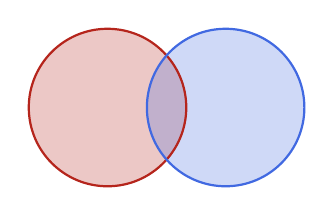
\begin{tikzpicture}[scale=0.5]
    \fill[BrickRed,fill opacity=0.25] (180:1.5) circle (2);
    \fill[RoyalBlue,fill opacity=0.25] (0:1.5) circle (2);
    \draw[BrickRed,thick] (180:1.5) circle (2);
    \draw[RoyalBlue,thick] (0:1.5) circle (2);
   \end{tikzpicture}
   \caption{Množiny $\clr{A}$ a $\clb{B}$.}
   \label{subfig:sjednoceni-a}
  \end{subfigure}
  \begin{subfigure}{.45\textwidth}
   \centering
   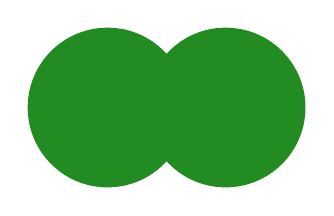
\begin{tikzpicture}[scale=0.5]
    \def\firstcircle{(180:1.5) circle (2)}
    \def\secondcircle{(0:1.5) circle (2)}
    \filldraw[thick,ForestGreen] \firstcircle; 
    \filldraw[thick,ForestGreen] \secondcircle;
   \end{tikzpicture}
   \caption{Sjednocení $\clg{A \cup B}$.}
   \label{subfig:sjednoceni-b}
  \end{subfigure}
  \caption{Operace sjednocení množin.}
  \label{fig:sjednoceni}
 \end{figure}
 \item \emph{průnikem} $A$ a $B$, zapsaným $A \cap B$, myslíme množinu
  obsahující pouze prvky ležící v obou množinách; logicky, $A \cap B$ je množina
  splňující
  \[
   (x \in A \cap B) \Leftrightarrow (x \in A \wedge x \in B).
  \]
  \begin{figure}[ht]
   \centering
   \begin{subfigure}{.45\textwidth}
    \centering
    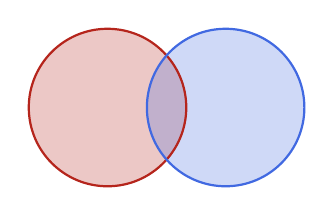
\begin{tikzpicture}[scale=0.5]
     \fill[BrickRed,fill opacity=0.25] (180:1.5) circle (2);
     \fill[RoyalBlue,fill opacity=0.25] (0:1.5) circle (2);
     \draw[BrickRed,thick] (180:1.5) circle (2);
     \draw[RoyalBlue,thick] (0:1.5) circle (2);
    \end{tikzpicture}
    \caption{Množiny $\clr{A}$ a $\clb{B}$.}
    \label{subfig:prunik-a}
   \end{subfigure}
   \begin{subfigure}{.45\textwidth}
    \centering
    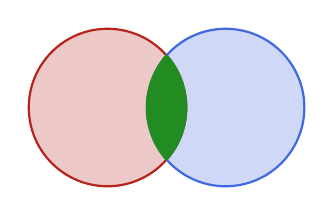
\begin{tikzpicture}[scale=0.5]
     \def\firstcircle{(180:1.5) circle (2)}
     \def\secondcircle{(0:1.5) circle (2)}
     
     \fill[BrickRed,fill opacity=0.25] \firstcircle;
     \fill[RoyalBlue,fill opacity=0.25] \secondcircle;
     \draw[BrickRed,thick] \firstcircle;
     \draw[RoyalBlue,thick] \secondcircle;

     \begin{scope}
      \clip \firstcircle;
      \fill[white] \secondcircle;
      \filldraw[thick,ForestGreen] \secondcircle;
     \end{scope}
     \begin{scope}
      \clip \secondcircle;
      \draw[ForestGreen,thick] \firstcircle;
     \end{scope}
    \end{tikzpicture}
    \caption{Průnik $\clg{A \cap B}$.}
    \label{subfig:prunik-b}
   \end{subfigure}
   \caption{Operace průniku množin.}
   \label{fig:prunik}
  \end{figure}
 \item \emph{rozdílem} $A$ a $B$, zapsaným $A \setminus B$, myslíme množinu
  obsahující prvky ležící v $A$, které však neleží v $B$; logicky, $A \setminus
  B$ je množina splňující
  \[
   (x \in A \setminus B) \Leftrightarrow (x \in A \wedge x \notin B).
  \]
  \begin{figure}[ht]
   \centering
   \begin{subfigure}{.3\textwidth}
    \centering
    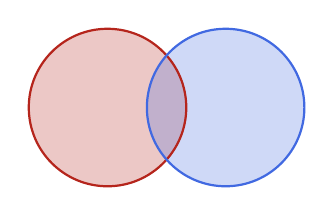
\begin{tikzpicture}[scale=0.5]
     \fill[BrickRed,fill opacity=0.25] (180:1.5) circle (2);
     \fill[RoyalBlue,fill opacity=0.25] (0:1.5) circle (2);
     \draw[BrickRed,thick] (180:1.5) circle (2);
     \draw[RoyalBlue,thick] (0:1.5) circle (2);
    \end{tikzpicture}
    \caption{Množiny $\clr{A}$ a $\clb{B}$.}
    \label{subfig:rozdil-a}
   \end{subfigure}
   \begin{subfigure}{.3\textwidth}
    \centering
    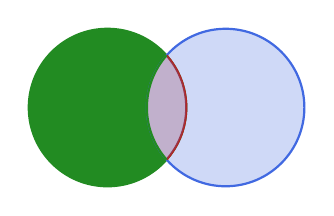
\begin{tikzpicture}[scale=0.5]
     \def\firstcircle{(180:1.5) circle (2)}
     \def\secondcircle{(0:1.5) circle (2)}
     
     \filldraw[thick,ForestGreen] \firstcircle;
     \fill[RoyalBlue,fill opacity=0.25] \secondcircle;
     \draw[RoyalBlue,thick] \secondcircle;

     \begin{scope}
      \clip \secondcircle;
      \fill[white] \firstcircle;
      \fill[BrickRed,fill opacity=0.25] \firstcircle;
      \draw[BrickRed,thick] \firstcircle;
     \end{scope}
     \begin{scope}
      \clip \firstcircle;
      \fill[RoyalBlue,fill opacity=0.25] \secondcircle;
      \draw[ForestGreen,thick] \secondcircle;
     \end{scope}
    \end{tikzpicture}
    \caption{Rozdíl $\clg{A \setminus B}$.}
    \label{subfig:rozdil-b}
   \end{subfigure}
   \begin{subfigure}{.3\textwidth}
    \centering
    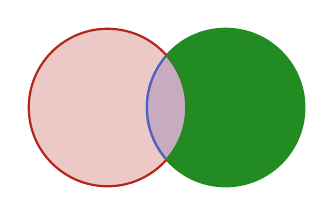
\begin{tikzpicture}[scale=0.5]
     \def\firstcircle{(0:1.5) circle (2)}
     \def\secondcircle{(180:1.5) circle (2)}
     
     \filldraw[thick,ForestGreen] \firstcircle;
     \fill[BrickRed,fill opacity=0.25] \secondcircle;
     \draw[BrickRed,thick] \secondcircle;

     \begin{scope}
      \clip \secondcircle;
      \fill[white] \firstcircle;
      \fill[RoyalBlue,fill opacity=0.25] \firstcircle;
      \draw[RoyalBlue,thick] \firstcircle;
     \end{scope}
     \begin{scope}
      \clip \firstcircle;
      \fill[BrickRed,fill opacity=0.25] \secondcircle;
      \draw[ForestGreen,thick] \secondcircle;
     \end{scope}
    \end{tikzpicture}
    \caption{Rozdíl $\clg{B \setminus A}$.}
    \label{subfig:rozdil-c}
   \end{subfigure}
   \caption{Operace rozdílu množin.}
   \label{fig:rozdil}
  \end{figure}
  Je dobré dbát faktu, že $A \setminus B$ a $B \setminus A$ jsou obecně
  \textbf{různé} množiny.
\end{itemize}

Operace sjednocení a průniku mají své \uv{hromadné} varianty, tedy sjednocení a
průnik většího (klidně nekonečného) počtu množin. V případech jako je tento, kdy
potřebujeme provádět operace na libovolném množství objektů, se často užívá
pomocné množiny, tzv. \emph{množiny indexů}, která slouží jen k tomu, aby
jednotlivé objekty v operované skupině od sebe odlišovala.

Konkrétně, zápisem
\[
 \bigcup_{i \in I} A_i,\text{ resp.}\bigcap_{i \in I} A_i,
\]
myslíme množinu, která obsahuje prvky, které leží aspoň v jedné, resp. v každé,
z množin $A_i,i \in I$, kde $I$ je libovolná množina indexů. K formální logické
definici je třeba použít kvantifikátorů, neboť množina $I$ nemusí mít konečně
prvků. Definujeme
\[
 (x \in \bigcup_{i \in I} A_i) \Leftrightarrow (\exists i \in I:x \in A_i)
\]
a
\[
 (x \in \bigcap_{i \in I} A_i) \Leftrightarrow ( \forall i \in I:x \in A_i).
\]
Tyto definice jsou původem matematické pranostiky \uv{Existenční kvantifikátor
je sjednocení a universální kvantifikátor je průnik.}

Ve speciálním případě, kdy $I = \{1,\ldots,n\}$ je množina přirozených čísel od
$1$ do $n$, se také užívá zápisů
\[
 \bigcup_{i = 1}^{n} A_i \quad \text{a} \quad \bigcap_{i = 1}^{n} A_i.
\]

Není obtížné si uvědomit, že pro rozdíl taková definice není možná, neboť u
rozdílu množin záleží na jejich pořadí a, opakujeme (vizte
\myref{výstrahu}{warn:mnozina-bez-poradi}), množina indexů $I$ \emph{neurčuje
pořadí}, v~kterém se množiny $A_i$ sjednocují či pronikají.

Dalším oblíbeným způsobem zápisu těchto operací, především v teorii kategorií,
je $\bigcup \mathcal{A}$ a $\bigcap \mathcal{A}$, kde $\mathcal{A} \coloneqq
\{A_i \mid i \in I\}$ je pomocná množina všech množin $A_i,i \in I$.
\textbf{Pozor!} Množina $\mathcal{A}$ není v~žádném smyslu sjednocením množin
$A_i$; je to množina, která má za prvky ony samotné množiny $A_i$, ne jejich
prvky. Obecně, žádný prvek žádné množiny $A_i$ není zároveň prvkem
$\mathcal{A}$, speciálně $A_i$ obecně \textbf{nejsou} podmnožiny $\mathcal{A}$.

\subsection{Kartézský součin a uspořádané n-tice}
\label{ssec:kartezsky-soucin-a-usporadane-n-tice}

Anobrž holý pojem množiny neobsahuje v žádném smyslu koncept \emph{pořadí}
prvku, je tento však pochopitelně užitečný, a proto si jej definujeme.

Zápisem $(x,y)$ myslíme tzv. \emph{uspořádanou dvojici} prvků $x$ a $y$. V této
dvojici je $x$ prvním prvkem a $y$ druhým. Je proto odlišná od množiny
$\{x,y\}$, protože $\{x,y\} = \{y,x\}$, ale $(x,y) \neq (y,x)$. V úvodu do této
kapitoly jsme tvrdili, že teorie množin tvoří svět matematiky. Pojem
\emph{dvojice}, který není shodný s pojmem \emph{množiny} tudíž musel bedlivé
čtenáře vylekat. Darmo se však lekati, uspořádané dvojice jsou rovněž množiny.
Než jej odhalíme, vybízíme čtenáře, aby našli způsob, kterak definovat
uspořádanou dvojici jako množinu.

Běžně užívaná definice (prve formulována Kazimierzem Kuratowskim) je
\[
 (x,y) \coloneqq \{\{x\},\{x,y\}\}.
\]
Ta říká, že uspořádaná dvojice $(x,y)$ je vlastně množina obsahující množinu s
jediným prvkem $x$ a množinu $\{x,y\}$. Ta je pak rozdílná od dvojice $(y,x)$,
což je množina $\{\{y\},\{x,y\}\}$. Tato definice je z~formálního hlediska
nutná, protože vytvářet matematické objekty nedefinovatelné v teorii množin rodí
chaos, ale intuitivně zcela nepoužitelná. Představme si dva lidi za sebou ve
frontě vnímat jako skupinu, v níž je skupina jenom s tím prvním a pak ještě
skupina obou. Tvrdíme, že je dobré udržet si pročež představu uspořádané dvojice
jakožto množiny, ve které mají navíc prvky svá pořadí.

Definice uspořádané dvojice se rekurzivně rozšíří na libovolný počet prvků.
Kupříkladu, uspořádanou trojici definujeme předpisem
\[
 (x,y,z) \coloneqq (x,(y,z)),
\]
to jest jako uspořádanou dvojici obsahující prvek $x$ a uspořádanou dvojici
$(y,z)$. Zápis pomocí množin se s rostoucím počtem prvků velmi rychle
komplikuje. Všimněte si, že už v drobném případě tří prvků dostaneme
\[
 (x,y,z) = (x,(y,z)) = (x,\{\{y\},\{y,z\}\}) = \{\{x\},\{x,
 \{\{y\},\{y,z\}\}\}\}.
\]
Máme-li $n$ prvků $x_1,\ldots,x_n$, pak jejich uspořádanou $n$-tici zapisujeme
$(x_1,\ldots,x_n)$.

Existence uspořádaných $n$-tic dává vzniknout jedné další množinové operaci --
kartézskému součinu. Kartézský součin dvou množin $A,B$, zapsaný $A \times B$,
definujeme jako množinu všech uspořádaných dvojic $(a,b)$, kde $a \in A$ a $b
\in B$. Název \emph{kartézský} (po Reném Descartesovi) ona nese pro zřejmou
souvislost se stejnojmenným systémem souřadnic. Totiž, souřadnice v rovině jsou
přesně dvojice $(x,y) \in \R \times \R$, kde $\R$ značí množinu reálných čísel.

Rovina skýtá navíc užitečný způsob přemýšlení o kartézském součinu jako o
\uv{dimenz\-ní} operaci. Má-li totiž $A$ dimenzi (v intuitivním slova smyslu)
$n$ a $B$ dimenzi $m$, pak $A \times B$ má dimenzi $n + m$. Například, je-li $A$
čtverec o délce strany $1$, pak $A^2 = A \times A$ je krychle o délce strany
$1$.

\begin{figure}[ht]
 \centering
 \begin{tikzpicture}[3d view,perspective,scale=1.5]
  \node (a11) at (0,0,0) {};
  \node (a12) at (0,-2,0) {};
  \node (a13) at (-2,-2,0) {};
  \node (a14) at (-2,0,0) {};
  
  \path [draw,BrickRed,thick,fill opacity=0.25,pattern=north east lines,pattern
   color=BrickRed] (a11.center) to (a12.center) to (a13.center) to (a14.center)
   to (a11.center);
  \node[circle,fill=white,inner sep=2pt] (a1label) at (-1,-1,0) {$\clr{A}$};

  \node (a21) at (0,0,0) {};
  \node (a22) at (0,-2,0) {};
  \node (a23) at (0,-2,2) {};
  \node (a24) at (0,0,2) {};
  
  \path [draw,RoyalBlue,thick,fill opacity=0.25,pattern=north east lines,pattern
   color=RoyalBlue] (a21.center) to (a22.center) to (a23.center) to (a24.center)
   to (a21.center);
  \node[circle,fill=white,inner sep=2pt] (a2label) at (0,-1,1) {$\clb{A}$};

  \node[vertex,BrickRed] (v1) at (-1,-0.5,0) {};
  
  \node[vertex,RoyalBlue] (v2) at (0,-0.5,1) {};
  \node[vertex,minimum size=9pt] (x) at (-1,-0.5,1) {};

  \draw[thick,dashed,BrickRed] (v1) -- (x);
  \draw[thick,dashed,RoyalBlue] (v2) -- (x);
  \node[left=1mm of x] {$(\clr{a_1},\clb{a_2})$};
  
 \end{tikzpicture}

 \caption{Vizualizace kartézského součinu $\clr{A} \times \clb{A}$.}
 \label{fig:kartezsky-soucin}
\end{figure}

Jakož tomu bylo i v případě sjednocení a průniku, lze definovat kartézský součin
více množin než dvou. Zde je však dlužen zřetel -- u kartézského součinu rovněž
(jako u rozdílu) záleží na pořadí násobení množin. Není možné definovat
kartézský součin množin $A_i$ pro libovolnou množinu indexů $I$, ale pouze pro
množinu \emph{uspořádanou} (tento pojem rovněž posléze připomeneme). Pro teď
budeme předpokládat, že $I = \{1,\ldots,n\}$ a zápisem
\[
 \prod_{i=1}^n A_i
\]
myslet množinu uspořádaných $n$-tic $(a_1,\ldots,a_n)$, kde $a_i \in A_i$ pro
každé $i \in \{1,\ldots,n\}$. Kartézský součin nekonečného množství množin lze
též definovat, ano akt to není přímočarý a naší věci zatím zbytečný.

Jsou-li všechny $A_i$, $i \in \{1,\ldots,n\}$, vskutku jednou množinou, $A$,
ujalo se -- poněkud přirozeně -- pro jejich kartézský součin mocninné značení.
To jest,
\[
 A^{n} \coloneqq \prod_{i = 1}^{n} A.
\]

\subsection{Relace}
\label{ssec:relace}

Relace, jak jejich název snad napovídá, jsou množiny, které kódují \emph{vztahy}
mezi prvky dvou různých množin. Jejich matematické pojetí je přímočaré a
elegantní, ano trochu neintuitivní. Totiž, relace (či \uv{vztah}) je zkrátka jen
výpis prvků, které v něm jsou, nikoli žádný nezávislý popis jeho vlastností.
Musíme-li načrtnout sociální rovnoběžku, můžeme si představit, že význam vztahu
přátelství je přesně určen seznamem všech párů přátel. I když ona rovnoběžka
vzbudila v mnohých čtenářích jistě značnou nedůvěru, taková definice vztahu v
matematice je jednoduchá a téměř nesrovnatelně užitečná.

\begin{definition}{Relace}{relace}
 Ať $A,B$ jsou množiny. \emph{Relací} $R$ mezi $A$ a $B$ míníme kteroukoli
 podmnožinu $R \subseteq A \times B$.
\end{definition}

Milí čtenáři se již jistě s několika relacemi setkali. Například samotný vztah
rovnosti ($=$) je relací. Podobně, vztahy \uv{býti menší nebo rovno} ($ \leq $)
či \uv{býti ostře větší} ($>$) jsou relacemi ve všech číselných oborech. Jak
tyto příklady naznačují, historicky se symboly relací píšou obvykle \emph{mezi}
prvky v oné relaci jsoucí. Tohoto úzu se držíme i my a pro relaci $R \subseteq A
\times B$ píšeme $aRb$, kdykoli $(a,b) \in R$. Jelikož je však zápis
$a\cancel{R}b$ poněkud neuhlazený a nadevše obtížně rozpoznatelný od svého
pozitivního protipólu, používáme množinové značení $(a,b) \notin R$, kdykoli
prvek $a$ není v relaci $R$ s prvkem $b$.

Máme-li k dispozici výčty prvků množin $A$ a $B$, je pro představu dobré kreslit
relace $R \subseteq A \times B$ do tzv. mříží. Ty tvoříme tak, že nakreslíme
doslovnou mříž teček s $\# A$ sloupci, resp. $\# B$ řádky, pro každý prvek
množiny $A$, resp. množiny $B$, a tečky na pozicích odpovídající párům $(a,b)
\in A \times B$, které rovněž leží v $R$, například kroužkujeme. Zvolíme-li
třeba
\[
 \clr{A} = \clr{\{1,2,3,4\}}, \clb{B} = \clb{\{a,b,c\}}
\]
a mezi nimi relaci
\[
 \clg{R} = \clg{\{(1,a),(1,b),(2,b),(3,a),(3,b),(3,c),(4,a)\}},
\]
bude jejím vyobrazením mříž na \myref{obrázku}{fig:mriz-relace}.

\begin{figure}[ht]
 \centering
 \begin{tikzpicture}
  \foreach \x in {1,2,3,4} {
   \foreach \y in {-1,-2,-3} {
    \node[vertex] at (\x,\y) {};
   }
  }
  \node (one) at (1,-0.5) {$\clr{1}$};
  \node (two) at (2,-0.5) {$\clr{2}$};
  \node (three) at (3,-0.5) {$\clr{3}$};
  \node (four) at (4,-0.5) {$\clr{4}$};
  \node (a) at (0.5,-1) {$\clb{a}$};
  \node (b) at (0.5,-2) {$\clb{b}$};
  \node (c) at (0.5,-3) {$\clb{c}$};
  
  \draw[ForestGreen,thick] (1,-1) circle (2mm);
  \draw[ForestGreen,thick] (1,-2) circle (2mm);
  \draw[ForestGreen,thick] (2,-2) circle (2mm);
  \draw[ForestGreen,thick] (3,-1) circle (2mm);
  \draw[ForestGreen,thick] (3,-2) circle (2mm);
  \draw[ForestGreen,thick] (3,-3) circle (2mm);
  \draw[ForestGreen,thick] (4,-1) circle (2mm);
 \end{tikzpicture}

 \caption{Mříž relace $\clg{R} \subseteq \clr{A} \times \clb{B}$.}
 \label{fig:mriz-relace}
\end{figure}

Relace zvláště zásadního významu jsou ty mezi dvěma totožnými množinami. Je-li
$R$ relace mezi $A$ a $A$ říkáme, výrazně lidštěji, že $R$ je relace \emph{na}
$A$. U relací na množině stavíme na piedestal ty s~jistými speciálními
vlastnostmi. Konkrétně, řekneme, že relace $R \subseteq A \times A$ je
\begin{itemize}
 \item \emph{reflexivní}, když je každý prvek v relaci $R$ sám se sebou, tj. $
  \forall x \in A:xRx$;
 \item \emph{antireflexivní}, když žádný prvek není v relaci $R$ sám se sebou,
  tj. $ \forall x:(x,x) \notin R$;
 \item \emph{symetrická}, když s každým párem prvků obsahuje i ten obrácený, tj.
  $ \forall x,y \in A:xRy \Rightarrow yRx$;
 \item \emph{antisymetrická}, když z každého páru dvojic $(x,y)$ a $(y,x)$ je v
  $R$ vždy jen jedna, tj. $ \forall x,y \in A: xRy \Rightarrow (y,x) \notin R$
  (všimněme si, že antisymetrická relace je automaticky antireflexivní);
 \item \emph{\textbf{slabě} antisymetrická}, když z každého páru dvojic $(x,y)$
  a $(y,x)$ je v $R$ vždy jen jedna za předpokladu, že $x$ a $y$ jsou od sebe
  různé, tj. $ \forall x,y \in A: (xRy \wedge yRx) \Rightarrow (x = y)$;
 \item \emph{transitivní}, když se přirozeně \uv{přenáší} přes prostřední prvek,
  tj. $ \forall x,y,z \in A:(xRy \wedge yRz) \Rightarrow xRz$.
\end{itemize}

\begin{figure}[ht]
 \centering
 \begin{subfigure}{.3\textwidth}
  \centering
  \begin{tikzpicture}[scale=0.75]
   \foreach \x in {1,2,3,4} {
    \foreach \y in {-1,-2,-3,-4} {
     \node[vertex] at (\x,\y) {};
    }
   }
   \foreach \x in {1,2,3,4} {
    \node at (\x,-0.25) {$\clr{\x}$};
   }
   \foreach \y in {1,2,3,4} {
    \node at (0.25,-\y) {$\clr{\y}$};
   }

   \foreach \x in {1,2,3,4} {
    \draw[ForestGreen,thick] (\x,-\x) circle (2.5mm);
   }
   \draw[ForestGreen,thick] (1,-3) circle (2.5mm);
   \draw[ForestGreen,thick] (2,-1) circle (2.5mm);
   \draw[ForestGreen,thick] (4,-2) circle (2.5mm);
   \draw[ForestGreen,thick] (3,-4) circle (2.5mm);
  \end{tikzpicture}
  \caption{Reflexivní a slabě antisymetrická, nikoli transitivní.}
  \label{subfig:relace-na-mnozine-a}
 \end{subfigure}
 \hfill
 \begin{subfigure}{.3\textwidth}
  \centering
  \begin{tikzpicture}[scale=0.75]
   \foreach \x in {1,2,3,4} {
    \foreach \y in {-1,-2,-3,-4} {
     \node[vertex] at (\x,\y) {};
    }
   }
   \foreach \x in {1,2,3,4} {
    \node at (\x,-0.25) {$\clr{\x}$};
   }
   \foreach \y in {1,2,3,4} {
    \node at (0.25,-\y) {$\clr{\y}$};
   }

   \draw[ForestGreen,thick] (1,-2) circle (2.5mm);
   \draw[ForestGreen,thick] (2,-1) circle (2.5mm);
   \draw[ForestGreen,thick] (1,-4) circle (2.5mm);
   \draw[ForestGreen,thick] (4,-1) circle (2.5mm);
   \draw[ForestGreen,thick] (2,-4) circle (2.5mm);
   \draw[ForestGreen,thick] (4,-2) circle (2.5mm);
  \end{tikzpicture}
  \caption{Antireflexivní, symetrická a transitivní.}
  \label{subfig:relace-na-mnozine-b}
 \end{subfigure}
 \hfill
 \begin{subfigure}{.3\textwidth}
  \centering
  \begin{tikzpicture}[scale=0.75]
   \foreach \x in {1,2,3,4} {
    \foreach \y in {-1,-2,-3,-4} {
     \node[vertex] at (\x,\y) {};
    }
   }
   \foreach \x in {1,2,3,4} {
    \node at (\x,-0.25) {$\clr{\x}$};
   }
   \foreach \y in {1,2,3,4} {
    \node at (0.25,-\y) {$\clr{\y}$};
   }

   \draw[ForestGreen,thick] (1,-2) circle (2.5mm);
   \draw[ForestGreen,thick] (1,-3) circle (2.5mm);
   \draw[ForestGreen,thick] (1,-4) circle (2.5mm);
   \draw[ForestGreen,thick] (2,-3) circle (2.5mm);
   \draw[ForestGreen,thick] (2,-4) circle (2.5mm);
   \draw[ForestGreen,thick] (3,-4) circle (2.5mm);
  \end{tikzpicture}
  \caption{Antisymetrická a transitivní (též \emph{ostré uspořádání}, zde $<$).}
  \label{subfig:relace-na-mnozine-c}
 \end{subfigure}
 \caption{Příklady relací $\clg{R}$ na množině $\clr{A} = \clr{\{1,2,3,4\}}$.}
 \label{fig:relace-na-mnozine}
\end{figure}

Naprosto klíčovými typy relací pro rozvoj další teorie jsou \emph{ekvivalence},
\emph{uspořádání} a \emph{zobrazení}. Každému typu je věnována jedna z
následujících sekcí.

\subsection{Relace ekvivalence}
\label{ssec:relace-ekvivalence}

Ekvivalence je relací na množině, která umožňuje dělit ji na části tvořené ve
smyslu daném touto relací \uv{stejnými}/ekvivalentními prvky. Ačkolivěk formálně
nemá \emph{relace} ekvivalence nic společného s \emph{logickou operací}
ekvivalence, důvody pro jejich jména souhlasí. Totiž, \emph{logická} ekvivalence
spojuje dva výroky, které jsou v pravdivostním smyslu stejné, a \emph{relační}
ekvivalence spojuje dva prvky množiny, které rovněž chceme (v daném kontextu)
považovat za totožné.

\begin{definition}{Relace ekvivalence}{relace-ekvivalence}
 Relaci $R$ na množině $A$ nazveme \emph{ekvivalencí}, pokud je
 \begin{itemize}
  \item reflexivní ($ \forall x \in A:xRx$),
  \item symetrická ($ \forall x,y \in A:xRy \Rightarrow yRx$),
  \item transitivní ($ \forall x,y,z \in A:(xRy \wedge yRz) \Rightarrow xRz$).
 \end{itemize}
\end{definition}
Spěšně si rozmyslíme smysluplnost této definice. Řekněme, že zkoumáme určité
vlastnosti lidí v~závislosti na jejich věku. Při takovéto studii pochopitelně
uvažujeme o dvou různých lidech stejného věku jako o \uv{totožných} subjektech.
Je samozřejmé, že dva skutečně stejné lidi považujeme za totožné (to vysvětluje
\emph{reflexivitu}). Podobně, když je člověk \emph{Jáchym} stejně starý jako
člověk \emph{Eric}, pak je i \emph{Eric} stejně starý jako \emph{Jáchym} (to
vysvětluje \emph{symetrii}). Konečně, když je člověk \emph{Lenin} stejně starý
jako člověk \emph{Stalin} a \emph{Stalin} je stejně starý jako \emph{Trotsky},
pak je přirozeně \emph{Lenin} stejně starý jako \emph{Trotsky} (to vysvětluje
\emph{transitivitu}).

Díky relaci \uv{býti stejného věku} můžeme nyní rozdělit množinu všech lidí na
Zemi na 122 (nejstarší zaznamenaný lidský věk) chlívků; v každém chlívku všichni
lidé stejně staří. Těmto \uv{chlívkům} se v matematice přezdívá \emph{třídy
ekvivalence}. Třídy ekvivalence $R$ na množině $A$ jsou podmnožiny $A$, kde
v~každé podmnožině jsou přesně jen ty prvky, které jsou spolu v relaci $R$.

\begin{definition}{Třída ekvivalence}{trida-ekvivalence}
 Ať $A$ je množina a $R$ ekvivalence na $A$. Vezměme $x \in A$. \emph{Třídou
 ekvivalence} prvku $x$ podle $R$, zapsanou $[x]_R$, myslíme množinu
 \[
  [x]_R \coloneqq \{y \in A \mid xRy\}
 \]
 všech prvků $y \in A$ v relaci $R$ s $x$. O podmnožině $X \subseteq A$ řekneme,
 že je to \emph{třída ekvivalence} $A$ podle $R$, když existuje prvek $x \in A$
 takový, že $X = [x]_R$.
\end{definition}

Jak lze snadno vyčíst z příkladu studie vlastností lidí stejného věku, každý
člověk je v právě jednom chlívku/třídě ekvivalence (jednomu člověku nemůže být
různý počet let, metabolický věk ignorujeme) a navíc každý člověk je nutně v
některém. Vladouce jazykem matematiky řčeme, že třídy ekvivalence dvou prvků
jsou buď stejné (oba lidé v témž chlívku), nebo disjunktní (každý člověk
v~různém chlívku). Navíc, sjednocením všech tříd ekvivalence dostaneme původní
množinu $A$, stejně jako spojením všech chlívků dostaneme jeden velký chlév s
batolaty i kmety na jedné hromadě. Tento fakt je platný pro každou ekvivalenci a
je oním klíčovým důvodem užitečnosti tohoto konceptu.

\begin{proposition}{O třídách ekvivalence}{o-tridach-ekvivalence}
 Ať $R$ je ekvivalence na $A$ a $X,Y$ jsou třídy ekvivalence $A$ podle $R$. Pak
 buď $X = Y$, nebo $X \cap Y = \emptyset$. Navíc, je-li 
 \[
  \mathcal{X} \coloneqq \{X \subseteq A\mid X \text{ třída ekvivalence } A
  \text{ podle } R\}
 \]
 množina všech (podle předchozí věty navzájem disjunktních) tříd ekvivalence
 množiny $A$ podle $R$, pak
 \[
  A = \bigcup \mathcal{X}.
 \]
\end{proposition}

Pro nějaký číselný příklad relace ekvivalence -- jenž zároveň ukazuje, že tříd
ekvivalence nemusí být konečně mnoho -- uvažme třeba relaci \uv{býti mocninou}
na přirozených číslech. Řekneme, že číslo $n \in \N$ je \emph{mocninou} $m \in
N$, když existuje kladné \textbf{racionální} (abychom mohli uvažovat i
odmocniny) číslo $q$ takové, že $n = m^{q}$. Taková relace je jistě ekvivalence,
neboť
\begin{itemize}
 \item $ \forall n \in \N: n = n^{1}$, tedy každé číslo je svou vlastní
  mocninou (reflexivita);
 \item když $n = m^{q}$, pak $m = n^{\frac{1}{q}}$, čili předpoklad, že $n$ je
  mocninou $m$, implikuje, že $m$ je mocninou $n$ (symetrie);
 \item když $n = m^{q_1}$ a $m = l^{q_2}$, pak $n = l^{q_1q_2}$, čili pokud je
  $n$ mocninou $m$ a $m$ mocninou $l$, pak $n$ je mocninou $l$ (transitivita).
\end{itemize}

\myref{Obrázek}{fig:tridy-ekvivalence-mocniny} zobrazuje prvních několik tříd
ekvivalence \uv{býti mocninou} na množině přirozených čísel.

\begin{figure}[ht]
 \centering
 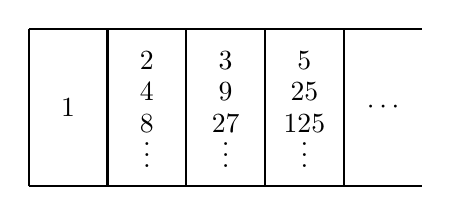
\begin{tikzpicture}
  \foreach \x in {0,1,2,3,4} {
    \draw[thick] (\x,0) -- (\x+1,0);
    \draw[thick] (\x,2) -- (\x+1,2);
    \draw[thick] (\x,0) -- (\x,2);
  }
  \node at (0.5,1) {$1$};

  \node at (1.5,1.6) {$2$};
  \node at (1.5,1.2) {$4$};
  \node at (1.5,0.8) {$8$};
  \node at (1.5,0.5) {$\vdots$};

  \node at (2.5,1.6) {$3$};
  \node at (2.5,1.2) {$9$};
  \node at (2.5,0.8) {$27$};
  \node at (2.5,0.5) {$\vdots$};
  
  \node at (3.5,1.6) {$5$};
  \node at (3.5,1.2) {$25$};
  \node at (3.5,0.8) {$125$};
  \node at (3.5,0.5) {$\vdots$};

  \node at (4.5,1) {$\cdots$};
  
 \end{tikzpicture}

 \caption{Třídy ekvivalence \uv{býti mocninou} na $\N$.}
 \label{fig:tridy-ekvivalence-mocniny}
\end{figure}

\subsection{Relace uspořádání}
\label{ssec:relace-usporadani}

V úvodu do \hyperref[sec:zakladni-pojmy-z-teorie-mnozin]{této sekce} jsme
zdůraznili fakt, že množiny \textbf{nejsou} v žádném smyslu uspořádané, tedy
nelze o jejich prvcích tvrdit, který jde první a poslední. Ovšem, čtenáři jsou
si jistě vědomi, že kupříkladu přirozená čísla uspořádána \emph{jsou} -- číslo
$1$ je menší než číslo $5$, $8$ větší než $3$. Tento výrok je však mírně
nepřesný. Samotná množina přirozených čísel uspořádaná \emph{není}, lze na ní
však definovat jistý všudypřítomný typ relace (v tomto případě $ \leq $) zvaný
\emph{uspořádání}. Definujeme si, které vlastnosti musí relace uspořádání na
množině mít.

\begin{definition}{Relace uspořádání}{relace-usporadani}
 Ať $A$ je množina a $R \subseteq A \times A$ je relace na $A$. Řekneme, že $R$
 je \emph{uspořádání} (někdy též nesoucí přívlastek \emph{neostré}), když je
 \begin{itemize}
  \item reflexivní (tj. $ \forall x \in A:xRx$),
  \item slabě antisymetrické (tj. $ \forall x,y \in A:(xRy \wedge yRx)
   \Rightarrow (x=y))$,
  \item transitivní (tj. $ \forall x,y,z \in A:(xRy \wedge yRz) \Rightarrow
   xRz)$.
 \end{itemize}
 Je-li naopak $R$ (silně) antisymetrické (tj. $ \forall x,y \in A:xRy
 \Rightarrow (y,x) \notin R$), a tudíž antireflexivní (tj. $ \forall x \in
 A:(x,x) \notin R$), řekneme, že je $R$ \emph{\textbf{ostré} uspořádání}.

 Je-li $A$ množina a $R$ (ostré) uspořádání na $A$, říkáme, že dvojice $(A,R)$ je
 \emph{(ostře) uspořádaná množina} (podle $R$).
\end{definition}

Zcela nejobyčejnější příklady (neostrých) uspořádání jsou relace $ \leq $ a $
\geq $ v číselných oborech. Vskut\-ku, každý prvek je menší/větší nebo roven sám
sobě, z každé dvojice prvek je buď jeden menší/větší než ten druhý, nebo jsou
stejné, a když je prvek $x$ menší/větší než prvek $y$ a ten zas menší/větší než
prvek $z$, pak je $x$ menší/větší než $z$. Speciálně, $(\N, \leq )$ a $(\N, \geq
)$ jsou uspořádané množiny.

Příkladem \emph{ostrých} uspořádání jsou relace $<$ a $>$, které se liší tím, že
žádný prvek není ostře menší/větší než on sám.

\begin{warning}{}{linearni-usporadani}
 Součástí definice uspořádání \textbf{není} podmínka, že \textbf{každé} dva
 prvky lze spolu porovnat. Pročež, v uspořádaných množinách obecně existují
 dvojice prvků, kde první není ani menší ani větší než ten druhý.

 Uspořádáním (ať už ostrým či neostrým) naopak \emph{splňujícím} onu podmínku
 říkáme \emph{lineární}.
\end{warning}

Za definicí uspořádání samozřejmě stojí myšlenka, že taková relace určuje
\emph{pořadí} prvků na množině. Z toho důvodu se obvykle uspořádání nekreslí
jako obecné relace do mříží, ale do tzv. Hasseho (po číselném teoretiku Helmutu
Hassem) diagramů, které získáme tím způsobem, že prvky nakreslíme jako puntíky a
každé dva puntíky prvků, které jsou v daném uspořádání porovnatelné, spojíme
úsečkou (nejsou-li již spojeny přes nějaký další puntík) a větší z nich
nakreslíme nad menší. Chováme na vědomí, že kreslit obrázky je více
uspokojující, než je popisovat, a tedy si závěrem této krátké sekce nakreslíme
(Hasseho diagramy) tři takřkouce \uv{učebnicové} příklady uspořádání.

\begin{example}{}{usporadani}
 \vspace{-\parskip}
 \begin{enumerate}
  \item Uvažme jednoduchý příklad uspořádané množiny $(\N, \leq )$. Už jsme si
   rozmysleli, že $ \leq $ je na $\N$ skutečně uspořádáním. Je triviální
   nahlédnout, že je rovněž lineární, neboť z~každých dvou přirozených čísel lze
   vybrat to menší.
  
   Lineární uspořádání mají velmi nezajímavý Hasseho diagram -- řetěz prvků,
   který může končit nahoře nebo dole. V tomto případě je nejmenším prvkem $0$ a
   nejvyšší neexistuje, tedy řetěz pokračuje nekonečně dlouho směrem nahoru.
   \begin{figure}[H]
    \centering
    \begin{tikzpicture}
     \foreach \y in {0,1,2,3} {
      \node[vertex] (v\y) at (0,\y) {};
      \node[right=1mm of v\y] {$\y$};
     }
     \foreach \y in {0,1,2} {
      \draw[thick] (0,\y) -- (0,\y+1);
     }
     \draw[thick] (0,3) -- (0,3.5);
     
     \node[above=5mm of v3] {$\vdots$};
    \end{tikzpicture}

    \caption{Hasseho diagram uspořádané množiny $(\N, \leq )$.}
    \label{fig:hasseho-diagram-N}
   \end{figure}
  \item O něco komplikovanější příklad je uspořádání inkluzí $ \subseteq $. Pro
   libovolnou množinu $A$ můžeme uvážit uspořádanou množinu $(2^{A}, \subseteq
   )$. Je téměř samozřejmé, že $ \subseteq $ je skutečně (neostré) uspořádání,
   které však \textbf{není} lineární. Vizme příklad.
  
   Ať $A \coloneqq \{1,2,3\}$. Pak jsou její podmnožiny $\{1,2\}$ a $\{2,3\}$
   neporovnatelné pomocí $ \subseteq $ -- ani jedna není podmnožinou té druhé.
   Zajímavým geometrickým faktem je, že Hasseho diagramem $(2^{A}, \subseteq )$
   pro $n$-prvkovou množinu $A$ je síť vrcholů krychle dimenze $n$.
   \begin{figure}[H]
    \centering
    \begin{tikzpicture}[scale=1.5]
     \node[vertex] (v0) at (0,0) {};
     \node[vertex] (v1) at (-1,1) {};
     \node[vertex] (v2) at (0,1) {};
     \node[vertex] (v3) at (1,1) {};
     \node[vertex] (v12) at (-1,2) {};
     \node[vertex] (v13) at (0,2) {};
     \node[vertex] (v23) at (1,2) {};
     \node[vertex] (v123) at (0,3) {};

     \draw[thick] (v0) -- (v1);
     \draw[thick] (v0) -- (v2);
     \draw[thick] (v0) -- (v3);
     \draw[thick] (v1) -- (v12);
     \draw[thick] (v1) -- (v13);
     \draw[thick] (v2) -- (v12);
     \draw[thick] (v2) -- (v23);
     \draw[thick] (v3) -- (v13);
     \draw[thick] (v3) -- (v23);
     \draw[thick] (v12) -- (v123);
     \draw[thick] (v13) -- (v123);
     \draw[thick] (v23) -- (v123);

     \node[below=0mm of v0] {$\emptyset$};
     \node[above=0mm of v123] {$\{1,2,3\}$};
     \node[below left=-1mm and -1mm of v1] {$\{1\}$};
     \node[below left=-1mm and -1mm of v2] {$\{2\}$};
     \node[below right=-1mm and -1mm of v3] {$\{3\}$};
     \node[above left=-1mm and -1mm of v12] {$\{1,2\}$};
     \node[above left=-1mm and -1mm of v13] {$\{1,3\}$};
     \node[above right=-1mm and -1mm of v23] {$\{2,3\}$};
    \end{tikzpicture}

    \caption{Hasseho diagram uspořádané množiny $(2^{A}, \subseteq )$ pro $A =
    \{1,2,3\}$.}
    \label{fig:hasseho-diagram-power-set}
   \end{figure}
 \end{enumerate}
\end{example}

\subsection{Relace zobrazení}
\label{ssec:relace-zobrazeni}

Přišel na řadu poslední klíčový typ relace, a pro algebraika snad nejdůležitější
myšlenka matematiky vůbec. Na rozdíl od relací uspořádání a ekvivalence, není
zobrazení nutně relace na téže množině. Jak název napovídá, zobrazení má něco
někam ... \uv{zobrazovat}. Matematik zřídkakdy přemýšlí o zobrazení jako o
relaci, nýbrž o popisu způsobu, kterak se prvky jedné množiny \uv{přetvářejí v}
či \uv{zobrazují na} prvky množiny druhé.

Zobrazení je dáno vlastně jednou přímočarou podmínkou -- každý prvek první
množiny se může zobrazit na maximálně jeden prvek množiny druhé. Lidově řečeno,
není prvku povoleno, aby se rozdvojil, roztřetil, rozčtvrtil, rozpětil,
rozšestil, rozsedmil, rozosmil, rozdevítil a indukcí dále.

Ať tedy $R$ je relace mezi $A$ a $B$. Elegantním logickým zápisem podmínky, aby
byl každý prvek $a \in A$ v relaci $R$ s \emph{maximálně jedním} prvkem $b \in
B$, je výrok, že jsou-li dva prvky z $A$ v relaci s týmž prvkem z $B$, pak se
vskutku jedná o jediný prvek. Formální definice následuje.

\begin{definition}{Zobrazení}{zobrazeni}
 Ať $R \subseteq A \times B$ je relace mezi $A$ a $B$. Nazveme $R$
 \emph{zobrazením} (z $A$ do $B$), pokud splňuje
 \[
  \forall a_1,a_2 \in A \; \forall b \in B: a_1Rb \wedge a_2Rb \Rightarrow a_1 =
  a_2.
 \]
 Zobrazení mezi množinami obvykle zapisujeme malými písmeny latinské abecedy
 počínaje písmenem $f$ (od \textbf{f}unkce, jak se některým speciálním typům
 zobrazení často říká). Fakt, že $f$ je zobrazení z $A$ do $B$, symbolizujeme
 zápisem $f:A \to B$ nebo též $A \overset{f}{ \longrightarrow } B$.

 Když $(a,b) \in f$, nepíšeme $afb$ jako u obecné relace, ale spíše $f(a) = b$
 či $f:a \mapsto b$.
\end{definition}

Stejně jako uspořádání, i zobrazení se kreslí svým osobitým způsobem, který v
sobě nese jejich mimořádnou povahu. Protože, opakujeme, bývají zobrazení vnímána
vlastně jako \uv{šipky} mezi množinami nesoucí prvky z první do té druhé, i se
tak kreslí. Konkrétně, zobrazení $f:A \to B$ nakreslíme například tak, že si
prvky $A$ postavíme nalevo, prvky $B$ napravo, a pro každý vztah $f(a) = b$
nakreslíme šipku z $a$ do $b$. Z definici zobrazení povede z každého $a \in A$
nejvýše jedna šipka. Vizte \myref{obrázek}{fig:priklady-zobrazeni}.

\begin{figure}[ht]
 \centering
 \begin{subfigure}[t]{.45\textwidth}
  \centering
  \begin{tikzpicture}
   \foreach \y in {1,2,3} {
    \node[vertex,BrickRed] (a\y) at (0,-\y) {};
    \node[left=0mm of a\y,BrickRed] {$\y$};
    
    \node[vertex,RoyalBlue] (b\y) at (2,-\y) {};
   }
   \node[vertex,BrickRed] (a4) at (0,-4) {};
   \node[left=0mm of a4,BrickRed] {$4$};

   \node[right=0mm of b1,RoyalBlue] {$a$};
   \node[right=0mm of b2,RoyalBlue] {$b$};
   \node[right=0mm of b3,RoyalBlue] {$c$};

   \draw[thick,ForestGreen,->,shorten <=2pt,shorten >=2pt] (a1) -- (b2);
   \draw[thick,ForestGreen,->,shorten <=2pt,shorten >=2pt] (a2) -- (b1);
   \draw[thick,ForestGreen,->,shorten <=2pt,shorten >=2pt] (a3) -- (b2);
   \draw[thick,ForestGreen,->,shorten <=2pt,shorten >=2pt] (a4) -- (b2);
  \end{tikzpicture}
  \caption{Zobrazení $\clg{f} =
  \{(\clr{1},\clb{b}),(\clr{2},\clb{a}),(\clr{3},\clb{b}),(\clr{4},\clb{b})\}$.}
  \label{subfig:priklady-zobrazeni-1}
 \end{subfigure}
 \begin{subfigure}[t]{.45\textwidth}
  \centering
  \begin{tikzpicture}
   \foreach \y in {1,2,3,4} {
    \node[vertex,BrickRed] (a\y) at (0,-\y) {};
    \node[vertex,BrickRed] (b\y) at (2,-\y) {};
    \node[left=0mm of a\y,BrickRed] {$\y$};
    \node[right=0mm of b\y,BrickRed] {$\y$};
   }

   \draw[thick,ForestGreen,->,shorten <=2pt,shorten >=2pt] (a1) -- (b2);
   \draw[thick,ForestGreen,->,shorten <=2pt,shorten >=2pt] (a2) -- (b3);
   \draw[thick,ForestGreen,->,shorten <=2pt,shorten >=2pt] (a3) -- (b1);
   \draw[thick,ForestGreen,->,shorten <=2pt,shorten >=2pt] (a4) -- (b4);
  \end{tikzpicture}
  \caption{Zobrazení $\clg{g} =
  \{(\clr{1},\clr{2}),(\clr{2},\clr{3}),(\clr{3},\clr{1}),(\clr{4},\clr{4})\}$.
 Zobrazením \uv{prohazujícím} prvky na množině se říká \emph{permutace}.}
  \label{subfig:priklady-zobrazeni-2}
 \end{subfigure}
 \caption{Příklady zobrazení.}
 \label{fig:priklady-zobrazeni}
\end{figure}

K zobrazením se tokem historie navázaly přehoušle názvosloví. Zopakujeme je zde,
bo pěstujeme zámysl je v dalším textu bez výstrah dštíti.

Ať $f$ do konce sekce značí zobrazení $A \to B$. Množinu $A$ nazýváme
\emph{doménou} zobrazení $f$, značíme $\dom f$, a množinu $B$ jeho
\emph{kodoménou}, značíme $\codom f$. Množinu všech prvků z $B$, na které se
zobrazuje nějaký prvek z $A$, nazýváme \emph{obrazem} $f$, značíme $\img f$.
Formálně
\[
 \img f \coloneqq \{b \in B \mid \exists a \in A: f(a) = b\}.
\]
Triviálně platí $\img f \subseteq \codom f$, ale tyto množiny nemusejí být
stejné. Například, zobrazení $\clg{f}$
z~\myref{obrázku}{subfig:priklady-zobrazeni-1} má obraz $\{\clb{a},\clb{b}\}$,
ale kodoménu celou množinu $\{\clb{a},\clb{b},\clb{c}\}$.

Pro každý prvek $b \in \codom f$ definujeme jeho \emph{vzor} (při zobrazení
$f$), značíme $f^{-1}(b)$, jako množinu \textbf{všech} prvků z $A$, které se na
něj zobrazují. Formálně, pro $b \in \codom f$
\[
 f^{-1}(b) \coloneqq \{a \in A \mid f(a) = b\}.
\]
Triviálně $f^{-1}(b) \subseteq \dom f$ pro každé $b \in \codom f$, ale tyto
množiny jistě mohou být různé. Pro zobrazení $\clg{f}$ z
\myref{obrázku}{subfig:priklady-zobrazeni-1} platí $\clg{f}^{-1}(\clb{b}) =
\{\clr{1},\clr{2},\clr{4}\}$ a $\clg{f}^{-1}(\clb{c})=\emptyset$ a pro zobrazení
$\clg{g}$ z \myref{obrázku}{subfig:priklady-zobrazeni-2} platí
$\clg{g}^{-1}(\clr{2}) = \{\clr{1}\}$. Přestože je vzor prvku při zobrazení
oficiálně \textbf{množina}, budeme v případech jako byl tento poslední, kdy je
vzorem množina jednoprvková, psát většinou $\clg{g}^{-1}(\clr{2}) = \clr{1}$ a
tvrdit, že prvek $\clr{1}$ je \emph{vzorem} prvku $\clr{2}$ při zobrazení
$\clg{g}$.

